\section{Flexbox: Konsep Container dan Item}

Flexbox (Flexible Box Layout) adalah model layout satu dimensi yang dirancang untuk mendistribusikan ruang dan menyelaraskan item di sepanjang satu sumbu---horizontal (baris) atau vertikal (kolom). Flexbox sangat cocok untuk komponen UI seperti navbar, card row, form controls, dan alignment vertikal yang sebelumnya sulit dicapai dengan CSS tradisional. Flexbox diaktifkan dengan \code{display: flex} pada kontainer; semua anak langsung menjadi \textbf{flex items} \cite{mdnCss}.

\begin{figure}[htbp]
\centering
\resizebox{0.85\textwidth}{!}{%
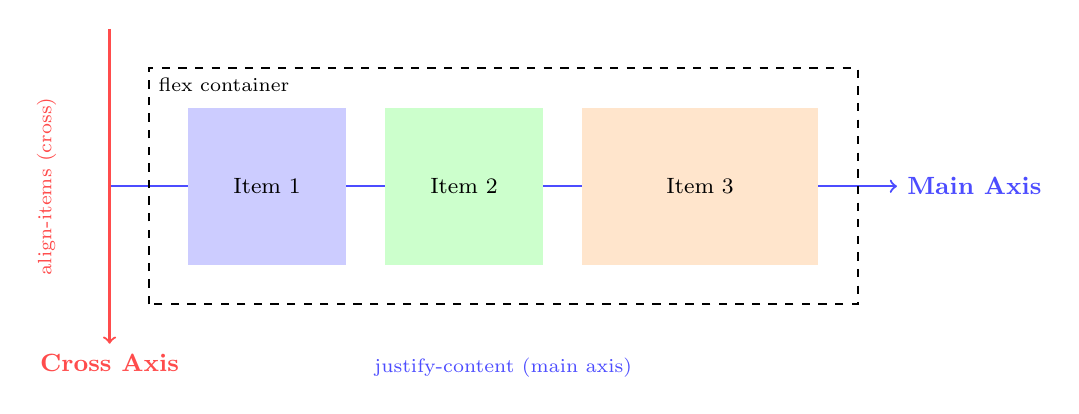
\begin{tikzpicture}[every node/.style={font=\footnotesize}]
  % Main axis
  \draw[->, thick, blue!70] (0,2) -- (10,2) node[right, font=\small\bfseries] {Main Axis};
  % Cross axis
  \draw[->, thick, red!70] (0,4) -- (0,0) node[below, font=\small\bfseries] {Cross Axis};
  % Container
  \draw[thick, dashed] (0.5,0.5) rectangle (9.5,3.5);
  \node[anchor=north west, font=\scriptsize] at (0.5,3.5) {flex container};
  % Items
  \fill[blue!20] (1,1) rectangle (3,3); \node at (2,2) {Item 1};
  \fill[green!20] (3.5,1) rectangle (5.5,3); \node at (4.5,2) {Item 2};
  \fill[orange!20] (6,1) rectangle (9,3); \node at (7.5,2) {Item 3};
  % Labels
  \node[font=\scriptsize, blue!70] at (5,-0.3) {justify-content (main axis)};
  \node[font=\scriptsize, red!70, rotate=90] at (-0.8,2) {align-items (cross)};
\end{tikzpicture}%
}
\caption{Sumbu Flexbox: main axis (horizontal) dan cross axis (vertikal)}
\end{figure}

\begin{table}[htbp]
\centering
\begin{tabular}{|P{3.5cm}|P{4cm}|P{4.5cm}|}
\hline
\textbf{Properti Container} & \textbf{Fungsi} & \textbf{Nilai Umum} \\
\hline
\code{flex-direction} & Arah main axis & \code{row}, \code{column}, \code{row-reverse} \\
\hline
\code{justify-content} & Distribusi di main axis & \code{flex-start}, \code{center}, \code{space-between}, \code{space-around} \\
\hline
\code{align-items} & Alignment di cross axis & \code{stretch}, \code{center}, \code{flex-start}, \code{flex-end} \\
\hline
\code{flex-wrap} & Wrap ke baris baru & \code{nowrap}, \code{wrap} \\
\hline
\code{gap} & Jarak antar item & \code{1rem}, \code{16px} \\
\hline
\end{tabular}
\caption{Properti utama flex container}
\end{table}

Flex items memiliki properti sendiri yang mengontrol perilaku individual. \code{flex-grow} menentukan proporsi perluasan jika ada ruang sisa (nilai 0 berarti tidak tumbuh, 1 berarti tumbuh proporsional). \code{flex-shrink} mengontrol penyusutan jika ruang tidak cukup. \code{flex-basis} menentukan ukuran awal sebelum distribusi ruang. Shorthand \code{flex: grow shrink basis} menggabungkan ketiganya; \code{flex: 1} setara dengan \code{flex: 1 1 0\%} (tumbuh dan susut proporsional) \cite{webdevCss}.

\begin{catatan}
\textbf{Flexbox vs Grid.} Flexbox bekerja di satu dimensi (baris ATAU kolom), sementara CSS Grid bekerja di dua dimensi (baris DAN kolom secara bersamaan). Gunakan Flexbox untuk komponen linear (navbar, toolbar, card row); gunakan Grid untuk layout halaman dan grid dua dimensi. Keduanya saling melengkapi dan dapat digunakan bersamaan \cite{cssTricks}.
\end{catatan}

